
\begin{figure}[t]
	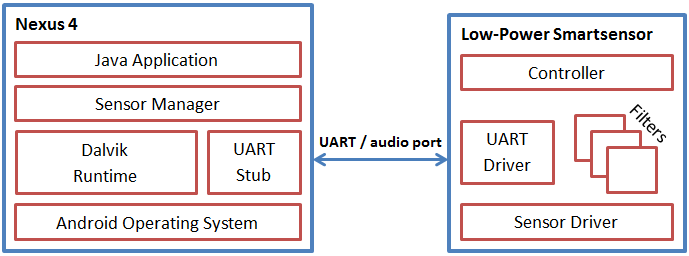
\includegraphics[width=9cm]{prototype_architecture.png}
	\caption{High-level Architecture of the Prototype (Nexus 4 and Smart Sensor board)}
    \label{fig:prototypeArchitecture}
\end{figure}

\section{Prototype}
\label{sec:prototype}

We implemented a prototype of our system using a Google Nexus 4 phone running Android 4.2.2. The low-power smart sensor is implemented using a Texas Instruments micro-controller board attached to an accelerometer sensor. The Nexus 4 and TI board communicate over the UART port made available by the Nexus 4 debugging interface via the physical port used by the audio interface. Figure \ref{fig:prototypeArchitecture} shows a high-level diagram of the prototype's architecture.

We chose to focus our efforts on the accelerometer sensor because of its relative simplicity and the availability of a wide range of accelerometer-based applications on various mobile application markets. Nevertheless, the approach can be extended to other low bit-rate sensors such as the microphone, GPS or WiFi. However, extending the prototype to work with higher bit-rate sensors like the camera would require a higher bandwidth data bus such as $I^2C$. 


\subsection{Google Nexus 4}
\label{subsec:nexus}

\begin{figure*}[t]
	\begin{verbatim}
		SensorManager mSensorManager = (SensorManager) getSystemService(Context.SENSOR_SERVICE);
		Sensor mAccelerometer = mSensorManager.getDefaultSensor(Sensor.TYPE_ACCELEROMETER);
		mSensorManager.registerListener(new MySensorEventListener(), mAccelerometer);
	\end{verbatim}
	\caption{Typical usage of Android's SensorManager}
    \label{fig:androidSensorCodeNormal}
\end{figure*}

\begin{figure*}[t]
	\begin{verbatim}
		SensorManager mSensorManager = (SensorManager) getSystemService(Context.SENSOR_SERVICE);
		Sensor mAccelerometer = mSensorManager.getDefaultSensor(Sensor.TYPE_ACCELEROMETER);
		DataFilterAlgorithm mDataFilter = new ExponentialMovingAverageLowPassFilter(0.75);
		WakeUpCondition mWakeUpCondition = new MinThresholdWakeUpCondition(mDataFilter, Sensor.AXIS_X, 12.0);
		mSensorManager.registerListener(new MySensorEventListener(), mAccelerometer, mWakeUpCondition);
	\end{verbatim}
	\caption{Usage of the SensorManager with a wakeup condition}
    \label{fig:androidSensorCodeModified}
\end{figure*}

On the Nexus phone we extended Android's SensorManager to include the new features made available by our system. To prevent a steep learning curve, our goal was to provide an API very similar to Android's existing sensors API. Normally, in order to receive sensor data, an application needs to register a listener (i.e. an implementation of the SensorEventListener interface) for a specific sensor with Android's SensorManager. Figure \ref{fig:androidSensorCodeNormal} shows a code example of a typical application registering a listener with the Android SensorManager for accelerometer readings. We extended the Sensor Manager to allow users to define custom wake-up conditions by specifying a pre-defined data filter and configuring the filter and wake-up parameters. The available types of wakeup conditions, described in detail in Subsection \ref{sec:sensorDataFilters}, are a set of predefined implementations of a DataFilterAlgorithm interface. Figure \ref{fig:androidSensorCodeModified} shows an example of the modified code to include an exponential moving average low pass filter with an alpha value of 75\% and a wakeup condition that is satisfied when the filtered x-axis acceleration exceeds $12\:m/s^2$.

We also created a UART stub to facilitate communication between the mobile phone and the smart sensor board. The UART stub is called when the smart sensor board detects an event based on its wakeup condition. In turn, the UART stub is a shell script that notifies the SensorManager using an Android Intent\cite{androidintents}.

For our prototype we avoid modifying the Android kernel in any way. Because the current prototype uses the UART port for communication with the smart sensor, we were able to constrain our implementation to the user space. An integrated implementation would likely make use of a higher bandwidth bus such as the $I^2C$ bus and require a custom driver and possibly modifications to the kernel.

\begin{table*}[t]
	\begin{tabular}{| p{7cm} | l | l |}
		\hline
		State & Average Power Consumption (mW) & Average Duration \\ \hline
	%    TI MSP430 & Awake & 3.6 & N/A \\ \hline
	%    TI Stellaris & Awake & 49.4 & N/A \\ \hline
		Awake, running a pedometer application with data from the internal accelerometer & 323 & N/A \\ \hline
		Asleep & 9.7 & N/A \\ \hline
		Asleep-to-Awake Transition & 384 & 1 second \\ \hline
		Awake-to-Asleep Transition & 341 & 1 second \\ \hline
	\end{tabular}
	\caption{Power Profile for the Google Nexus 4}
	\label{table:powerProfileNexus}
\end{table*}

We power profiled the Google Nexus 4. The results are summarized in Table \ref{table:powerProfileNexus}. During all the measurements, the device's screen was turned off. Additionally, we noticed that changes in signal strength for GSM, WiFi and GPS resulted in fluctuations in the power consumption of the device. To prevent these factors from affecting our power profile, we decided to run all the power measurements with GSM, WiFi and GPS turned off. While the device is sleeping, its power usage is very low, consuming only 9.7 mW. While awake, the power consumption is significantly higher, averaging 323 mW. During our power measurements we noticed that additional energy is consumed during transitions between the asleep and awake states. Each transition takes about 1 second. During a wakeup transition, the average power consumption goes up to 384 mW, while during an awake-to-asleep transition the average power consumption is 341 mW.

\todo[inline]{TODO for Wilson: we probably need a section that describes how the UART stub opens a serial port and then uses a TTY to copy the sensor readings and start the shell script that notifies the sensor manager. Talk about the bandwidth that we get and how long it takes us to copy sensor readings.}

\subsection{Smart Sensor Board}
\label{subsec:sensorBoard}

On the low-power smart sensor board, the prototype consists of a driver that talks to the accelerometer sensor, a set of filtering algorithms, a controller, and an UART driver for communicating with the phone. The controller orchestrates the execution of the filters, and uses the UART driver to wake up the phone when a wakeup condition is satisfied.

\subsubsection{Sensor Data Filters}
\label{sec:sensorDataFilters}

Accelerometer sensor data is particularly noisy. As a result many applications using this kind of data implement low-pass filters to remove noise and "smooth out" the accelerometer readings. On our Smart Sensor board we implemented three types of sensor data filters of varying complexities. 

The \textbf{Null Filter} algorithm is the simplest and requires no additional computation. This algorithm performs no filtering (i.e. the output sensor data is the same as the input sensor data). We use this "filter" to pass raw accelerometer readings to algorithms down the pipeline.

The \textbf{Exponential Moving Average Low-Pass Filter} (EMA-LPF) removes some of the noise from the sensor data and is computationally cheap, requiring only a few algebraic operations for every sensor reading. This filter takes an alpha parameter between 0 and 1, that controls the ``smoothness'' of the filtered data. This filter can be described using the following equation:

$output\:reading = $

$ = (1-\alpha) \times last\:output\:reading + \alpha \times input\:reading$

The \textbf{Fast Fourier Transformation based low-pass filter}~\cite{libbyFootstepDetection} (FFT-LPF) is more accurate at removing noise from the sensor data. However, it is computationally expensive. Two parameters can be set for the FFT-LPF: a window-size and a relative energy threshold value. The window size indicates the number of readings that are to be used in each discrete Fourier transform. The relative energy threshold value controls the amount of energy in the output data. A lower relative energy threshold value would result in ``smoother'' output sensor values.

\subsubsection{Wake-up conditions}

In our prototype, a wake-up condition comprises of a sensor data filter as described in the previous section and a set of wake-up parameters. This set contains the type of threshold to be used and the threshold value(s). We implemented three similar types of thresholds:

\begin{itemize}
\setlength{\itemsep}{-3pt}  

\item A \textbf{Minimum Threshold} that is satisfied when the acceleration exceeds the threshold value

\item A \textbf{Maximum Threshold} that is satisfied when the acceleration goes below the threshold value

\item A \textbf{Threshold Range} that is satisfied when the acceleration is between two threshold values

\end{itemize}

\subsubsection{Hardware Options}
\todo[inline]{TODO for Wilson: We need to talk about the actual sensor used by the board.}
We evaluated two options for our low-powered sensor platform. 

Our first option is a Texas Instruments MSP430 micro-controller. It has the advantage of requiring very little power, consuming only 3.6 mW while awake. However, it has limited memory and cannot perform complex analysis of sensor data in real-time. In our tests, the MSP430 was unable to run the Fast Fourier Transformations necessary for low-pass filtering sensor data in real-time. 

Our second option is a Texas Instruments Stellaris LM4F120H5QR micro-controller powered by a Cortex-M4 processor. It can batch a higher number of accelerometer readings and run all our wakeup conditions in real-time, including the one using FFT-based low-pass filtering. However, this micro-controller has an energy footprint an order of magnitude greater than the MSP430, consuming an average of 49.4 mW while awake.


